\chapter{Mass fit to \decay{\Bp}{\Dsp\phiz} candidates} 
\label{ch:B2DsPhi}

\minitoc

In this chapter the methodology used to search for \decay{\Bp}{\Dsp\phiz} decays is described.

{\color{Red}
\begin{itemize}
\item Details of blinding procedure for historic context
\end{itemize}
}

\section{Fit components}
\label{sec:B2DsPhi_fitcomponents}


\subsection{Signal decays}
\label{sec:B2DsPhi_signalcomps}

%%%%%%%%%%%%%%%%%%%%%%%%%%%%%%%%%%%%%%%%%%%%%%%%%%%%%%%%%% 
\begin{table}[h]
\centering
\begin{tabular}{ c c c c }
\hline
\multirow{2}{*}{Parameter}                   & \multicolumn{3}{c} {Value} \\
\cline{2-4}
                            & \decay{\Dsp}{\Kp\Km\pip}   & \decay{\Dsp}{\Kp\pim\pip} & \decay{\Dsp}{\pip\pim\pip}  \\
\hline
%\textbf{$\B \to \Ds \phi$}  &                    &                    &                        \\
\multicolumn{4}{l} {\decay{\Bp}{\Dsp\phiz}}\\

\hline
$\sigma_1/\sigma_2$         & 0.49 $\pm$ 0.01    & 0.47 $\pm$ 0.01    & 0.46 $\pm$ 0.01        \\
$f_\sigma$                  & 0.80 $\pm$ 0.01    & 0.84 $\pm$ 0.01    & 0.81 $\pm$ 0.01        \\
$\alpha$                    & 2.76 $\pm$ 0.07    & 3.06 $\pm$ 0.16    & 3.71 $\pm$ 0.23        \\
$n$                         & 1 $\pm$ 0          & 1  $\pm$ 0         & 1  $\pm$ 0             \\
\hline
%\textbf{ }  &                    &                    &                        \\
\multicolumn{4}{l} {\decay{\Bp}{\Dsp\Dzb}}\\
\hline
$\sigma_1/\sigma_2$         & 0.43 $\pm$ 0.01    & 0.42 $\pm$ 0.01    & 0.40 $\pm$ 0.01        \\
$f_\sigma$                  & 0.88 $\pm$ 0.01    & 0.88 $\pm$ 0.01    & 0.88 $\pm$ 0.01        \\
$\alpha$                    & 2.91 $\pm$ 0.06    & 3.36 $\pm$ 0.26    & 3.53 $\pm$ 0.25        \\
$n$                         & 1 $\pm$ 0          & 1 $\pm$ 0          & 1 $\pm$ 0              \\
\hline 
$\sigma_{1}(\Dsp\phi) / \sigma_{1}(\Dsp\Dzb)$ & 1.27 $\pm$ 0.02 & 1.31 $\pm$ 0.02 & 1.26 $\pm$ 0.02 \\
\hline

\end{tabular}
\caption{Fixed values obtained in fits to MC used in the model for the signal pdf.} 
\label{tab:mc_fits}  
\end{table}
%%%%%%%%%%%%%%%%%%%%%%%%%%%%%%%%%%%%%%%%%%%%%%%%%%%%%%%%%% 

%%%%%%%%%%%%%%%%%%%%%%%%%%%%%%%%%%%%%%%%%%%%%%%%%%%%%%%%%%
\begin{figure}[!h]
    \centering
    \begin{subfigure}[t]{1.0\textwidth}
        \includegraphics[width=0.48\textwidth]{figs/B2DsPhi/Plot_signal_Fit_All_B2PhiDs_Ds2KKPi.pdf}
        \includegraphics[width=0.48\textwidth]{figs/B2DsPhi/Plot_signal_Fit_All_B2D0Ds_Ds2KKPi.pdf}
        \caption{\decay{\Dsp}{\Kp\Km\pip}}
    \end{subfigure}\\
    \begin{subfigure}[t]{1.0\textwidth}
        \includegraphics[width=0.48\textwidth]{figs/B2DsPhi/Plot_signal_Fit_All_B2PhiDs_Ds2KPiPi.pdf}
        \includegraphics[width=0.48\textwidth]{figs/B2DsPhi/Plot_signal_Fit_All_B2D0Ds_Ds2KPiPi.pdf}
        \caption{\decay{\Dsp}{\Kp\pim\pip}}
    \end{subfigure}\\
    \begin{subfigure}[t]{1.0\textwidth}
        \includegraphics[width=0.48\textwidth]{figs/B2DsPhi/Plot_signal_Fit_All_B2PhiDs_Ds2PiPiPi.pdf}
        \includegraphics[width=0.48\textwidth]{figs/B2DsPhi/Plot_signal_Fit_All_B2D0Ds_Ds2PiPiPi.pdf}
        \caption{\decay{\Dsp}{\pip\pim\pip}}
    \end{subfigure}\\
    \caption{Invariant mass fits to signal (left) and normalisation (right) channel simulation samples.}
    \label{fig:B2DsPhi_signal_fits}   
\end{figure}
%%%%%%%%%%%%%%%%%%%%%%%%%%%%%%%%%%%%%%%%%%%%%%%%%%%%%%%%%%


{\color{Red}
\begin{itemize}
\item plots of signal shapes
\end{itemize}
}



\subsection{Partially reconstructed backgrounds}
\label{sec:B2DsPhi_partrecocomps}

%%%%%%%%%%%%%%%%%%%%%%%%%%%%%%%%%%%%%%%%%%%%%%%%%%%%%%%%%%
\begin{figure}[!h]
    \centering
    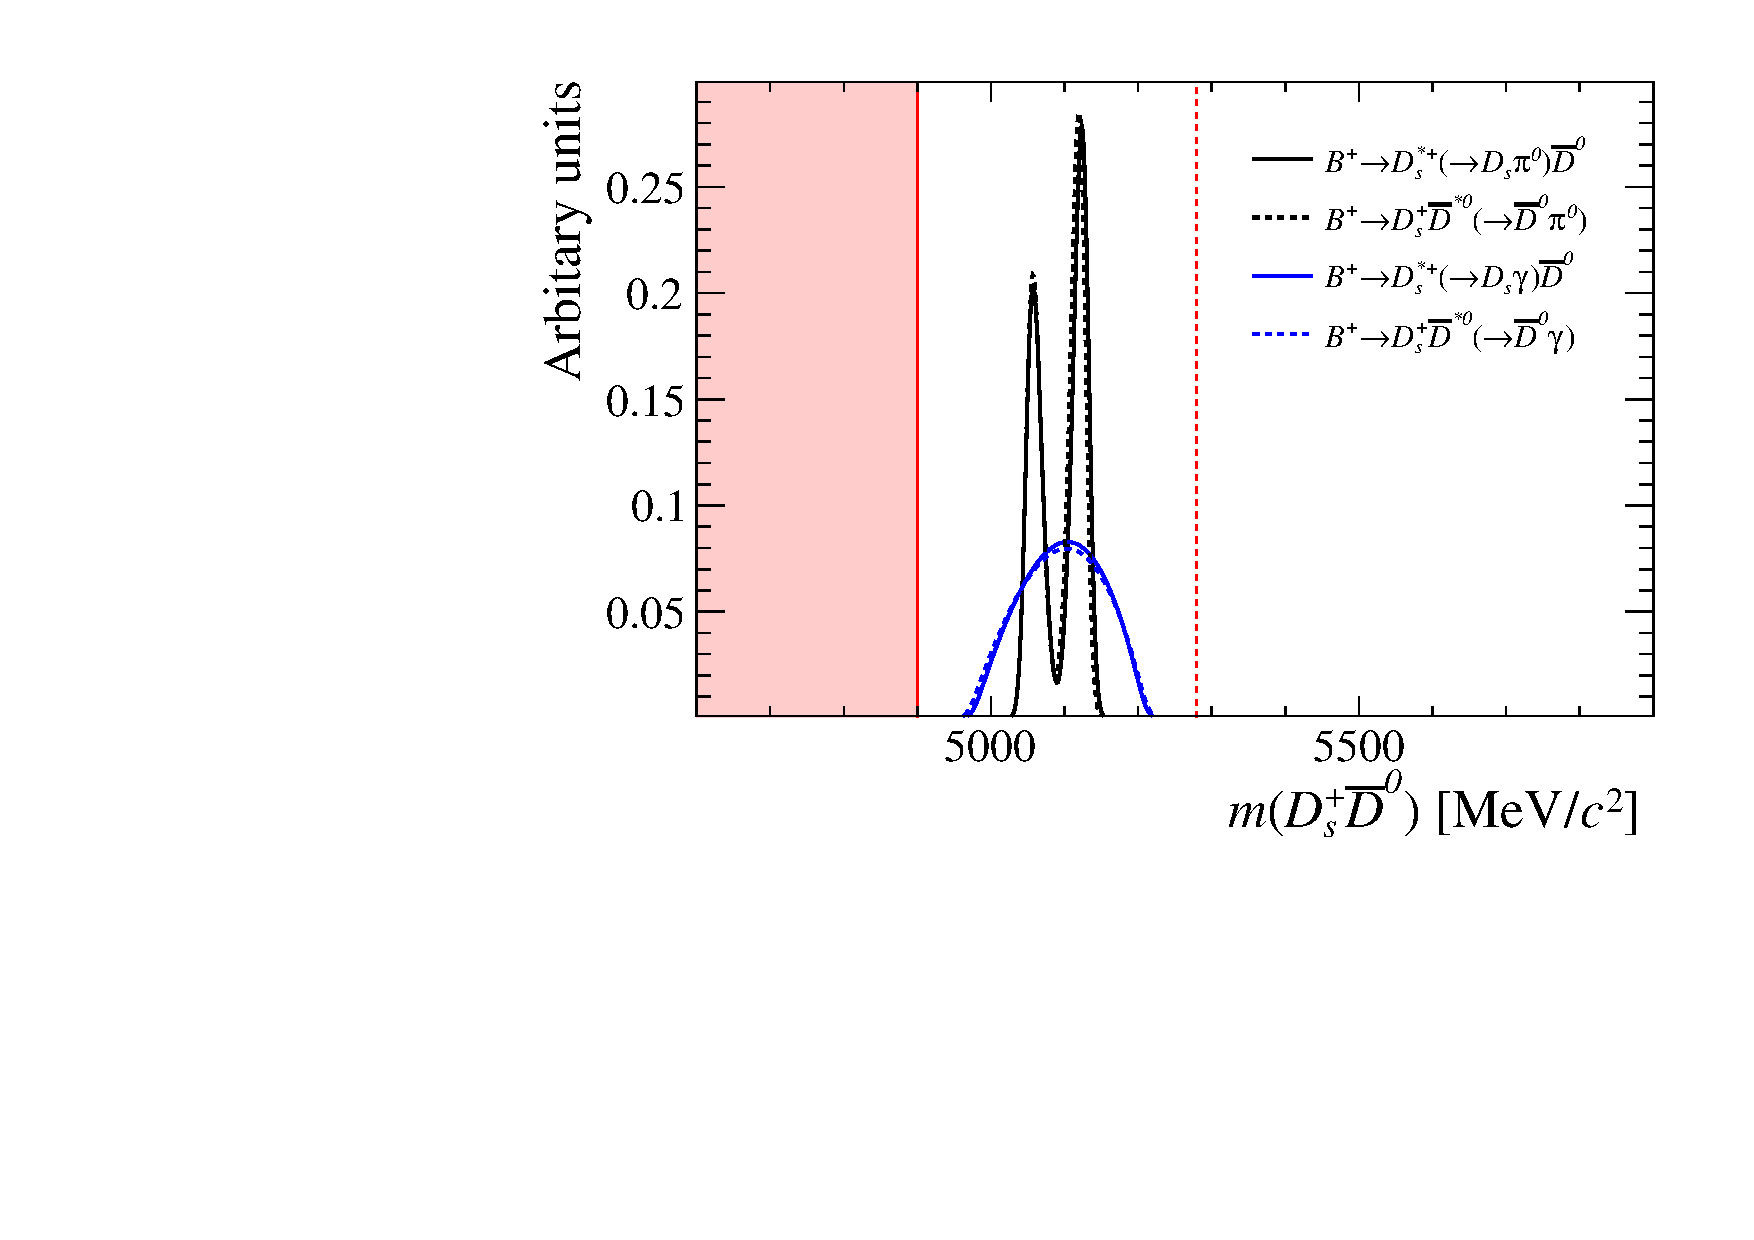
\includegraphics[width=0.60\textwidth]{figs/B2DsPhi/DsD0_part_reco_Shapes.pdf}
    \caption{Partially reconstructed \Dsp\Dzb shapes.}
    \label{fig:B2DsPhi_DsD0_partreco}   
\end{figure}
%%%%%%%%%%%%%%%%%%%%%%%%%%%%%%%%%%%%%%%%%%%%%%%%%%%%%%%%%%


%%%%%%%%%%%%%%%%%%%%%%%%%%%%%%%%%%%%%%%%%%%%%%%%%%%%%%%%%%
\begin{figure}[!h]
    \centering
    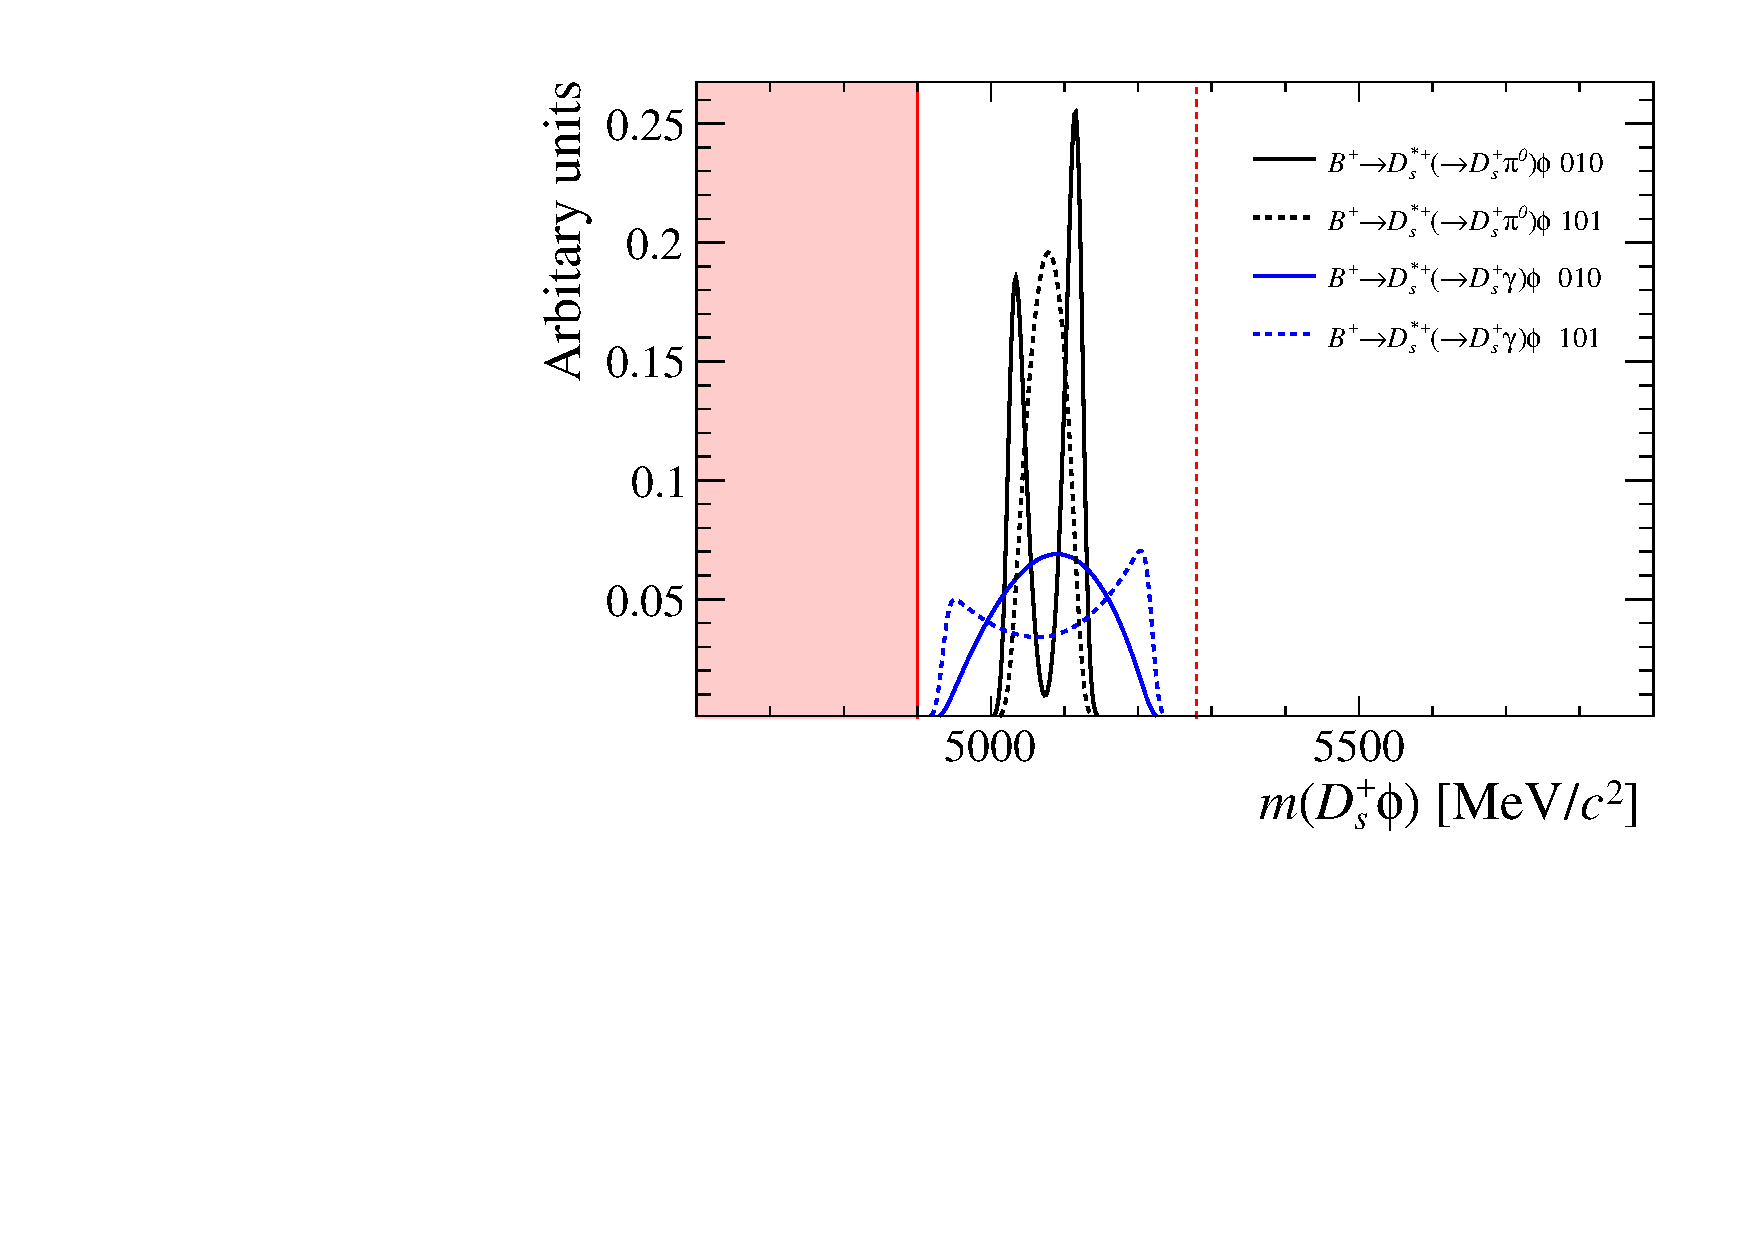
\includegraphics[width=0.60\textwidth]{figs/B2DsPhi/DsPhi_part_reco_Shapes.pdf}
    \caption{Partially reconstructed \Dsp\phiz shapes.}
    \label{fig:B2DsPhi_DsPhi_partreco}   
\end{figure}
%%%%%%%%%%%%%%%%%%%%%%%%%%%%%%%%%%%%%%%%%%%%%%%%%%%%%%%%%%


%%%%%%%%%%%%%%%%%%%%%%%%%%%%%%%%%%%%%%%%%%%%%%%%%%%%%%%%%%
\begin{figure}[!h]
    \centering
    \begin{subfigure}[t]{0.49\textwidth}
        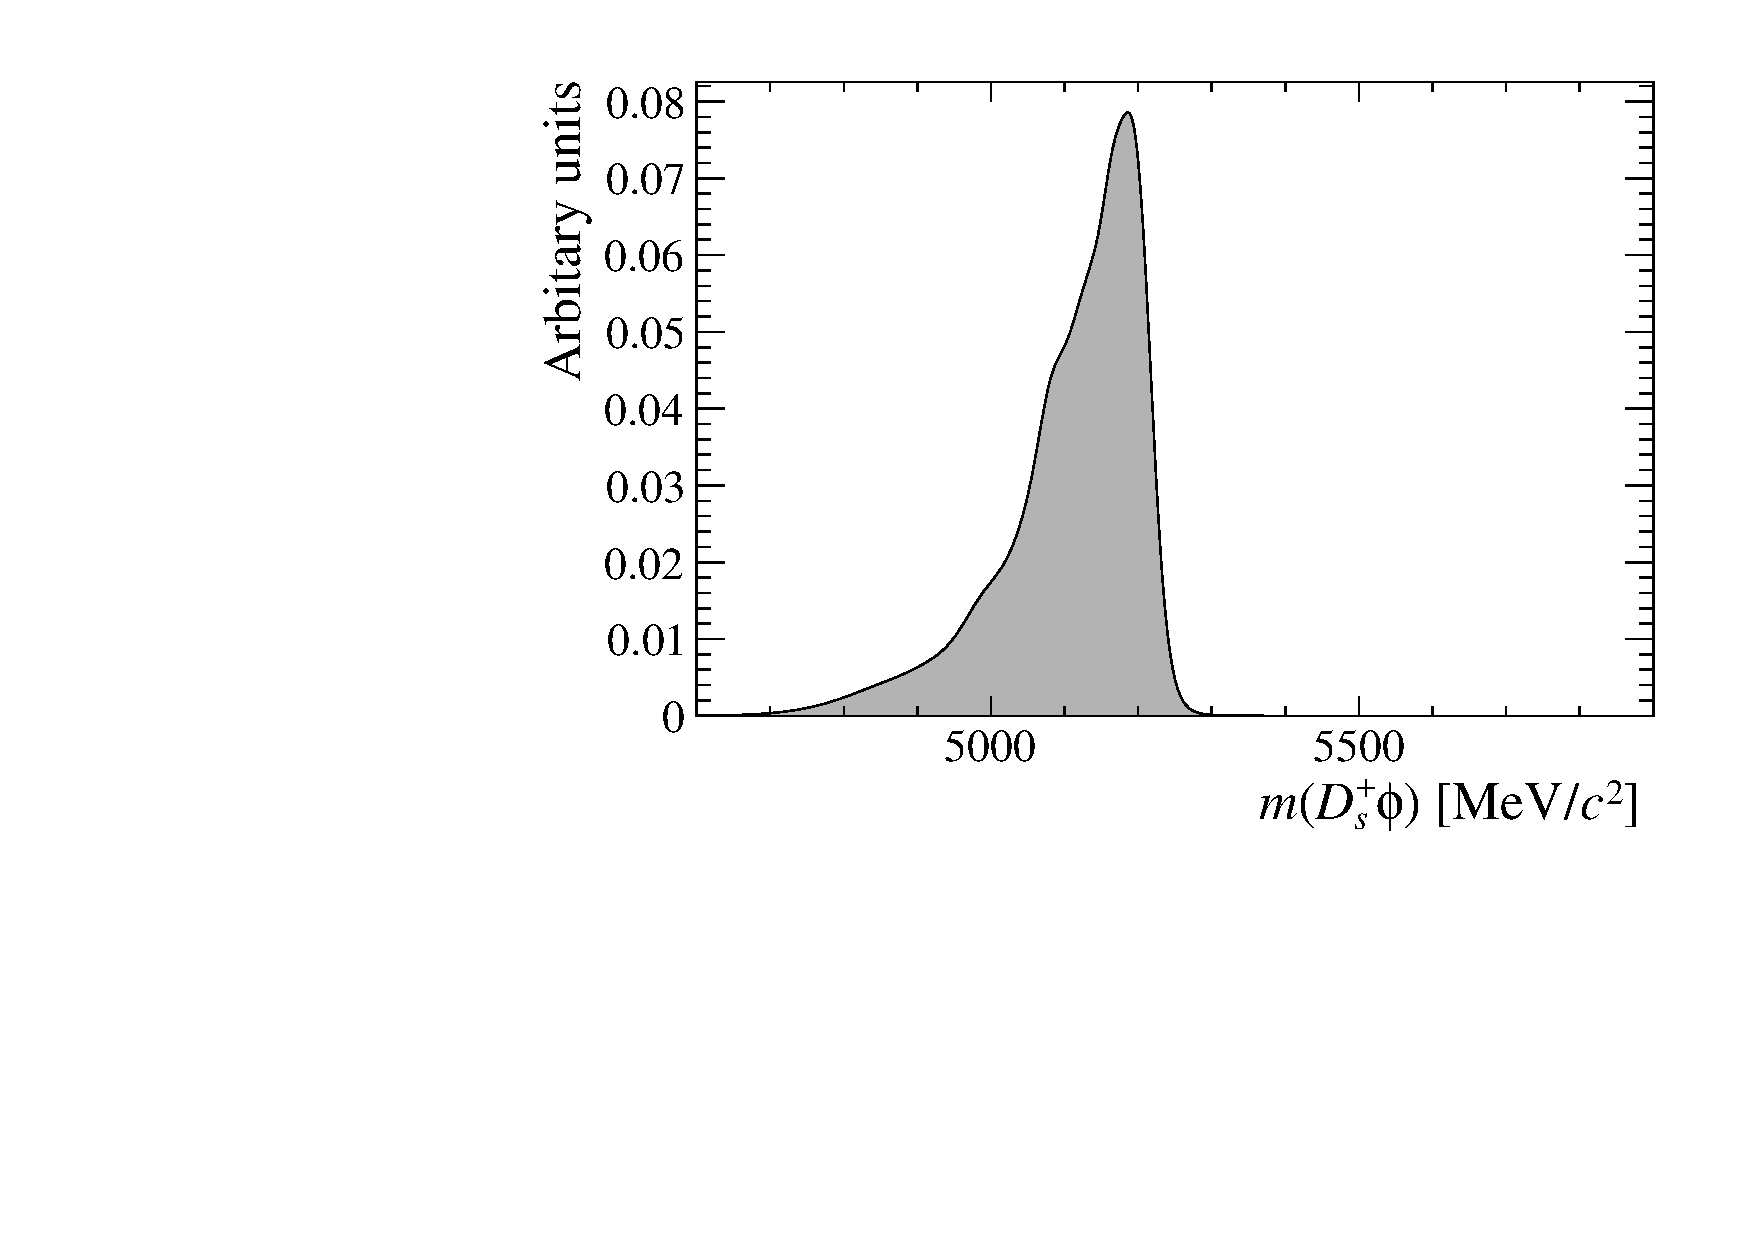
\includegraphics[width=1.0\textwidth]{figs/B2DsPhi/Bs2Dsa1_4600_5900_Shape.pdf}
        \caption{\decay{\Bsb}{\Dsp} }
    \end{subfigure}
    \begin{subfigure}[t]{0.49\textwidth}
        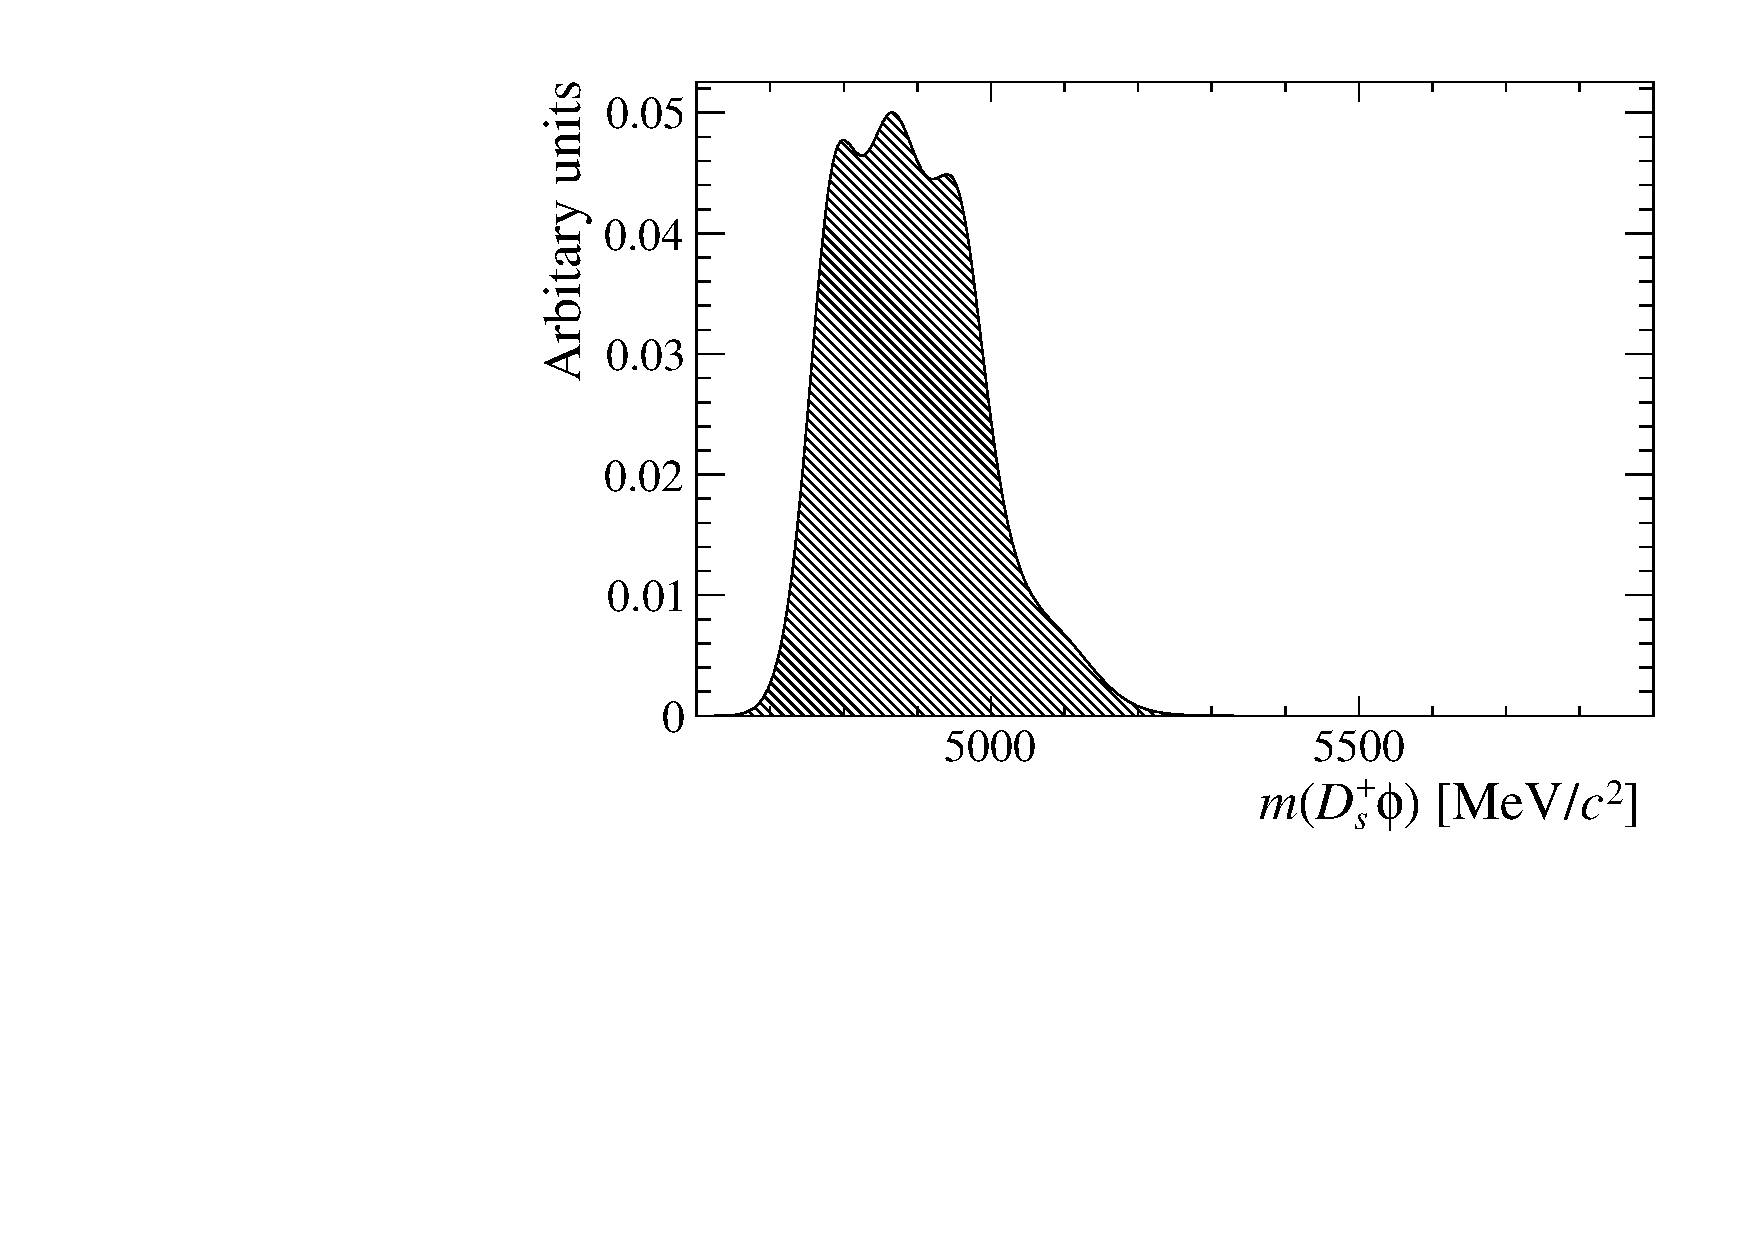
\includegraphics[width=1.0\textwidth]{figs/B2DsPhi/Bs2DsstKKst_4600_5900_Shape.pdf}
        \caption{\decay{\Bsb}{\Dsp\Kstar\Kp} }
    \end{subfigure}
    \begin{subfigure}[t]{0.49\textwidth}
        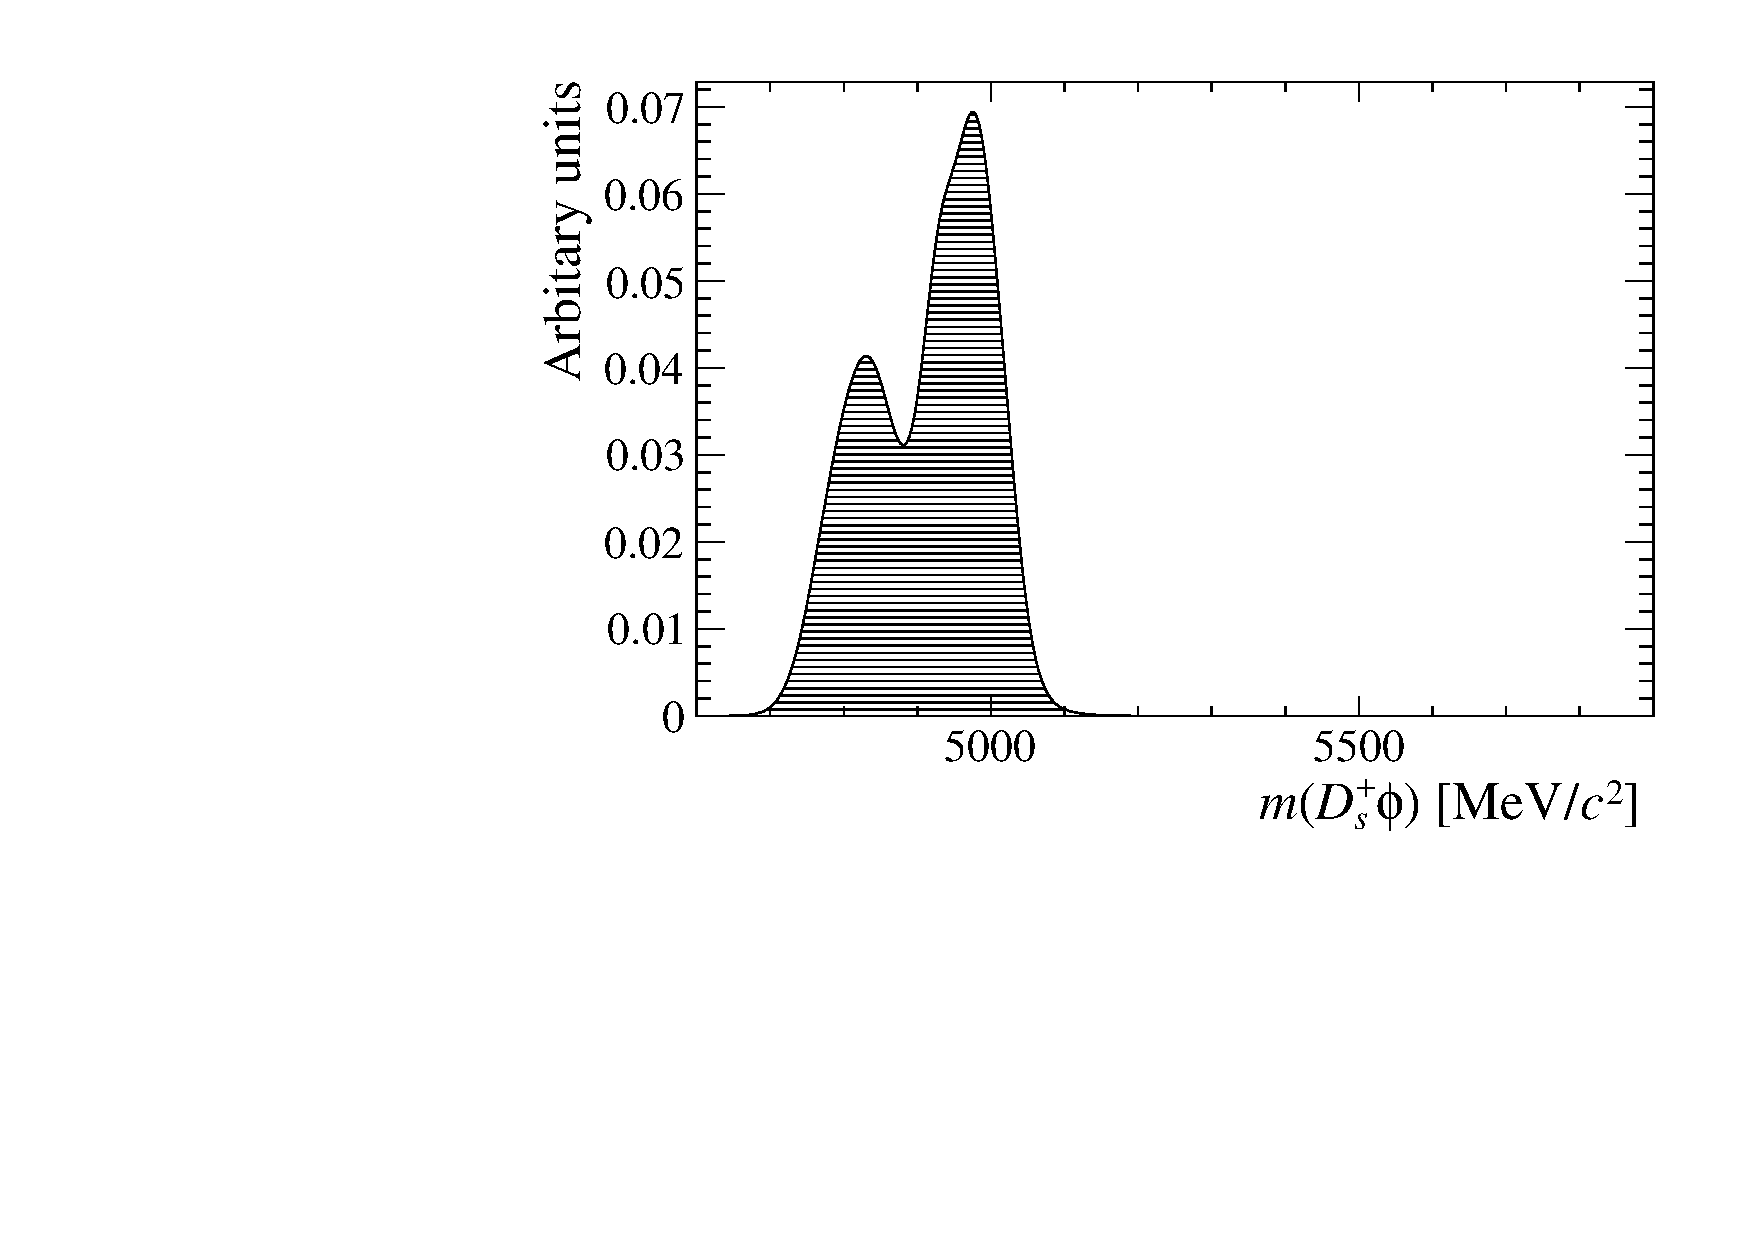
\includegraphics[width=1.0\textwidth]{figs/B2DsPhi/Bs2DsDs_4600_5900_Shape.pdf}
        \caption{\decay{\Bsb}{\Dsp\Dsm} }
    \end{subfigure}
    \begin{subfigure}[t]{0.49\textwidth}
        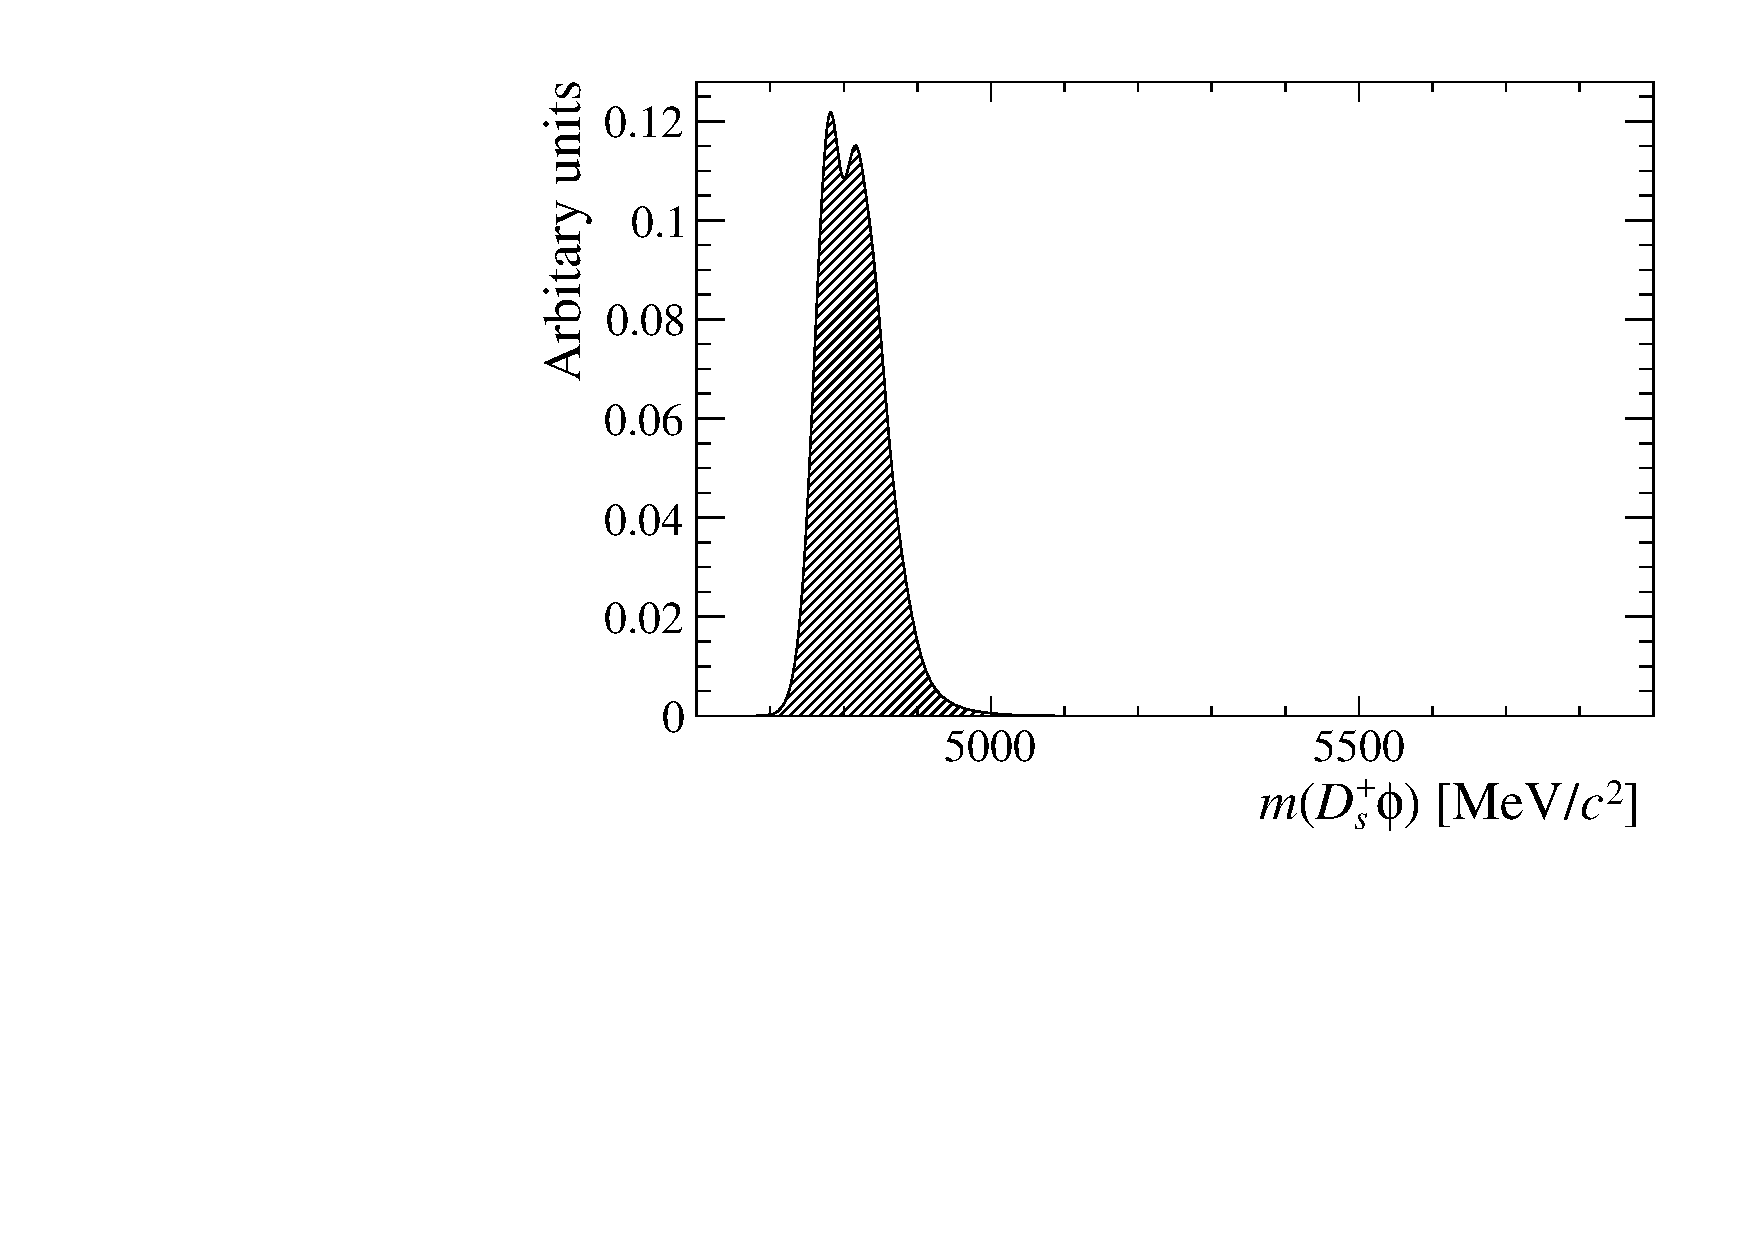
\includegraphics[width=1.0\textwidth]{figs/B2DsPhi/Bs2DsstDs_4600_5900_Shape.pdf}
        \caption{\decay{\Bsb}{\Dssp\Dsm} }
    \end{subfigure}
    \caption{Partially reconstructed mass shapes}
    \label{fig:B2DsPhi_signal_fits}   
\end{figure}
%%%%%%%%%%%%%%%%%%%%%%%%%%%%%%%%%%%%%%%%%%%%%%%%%%%%%%%%%%

{\color{Red}
\begin{itemize}
\item plots of partreco shapes
\end{itemize}
}

\subsection{Combinatorial  backgrounds}
\label{sec:B2DsPhi_combcomps}



\section{Fit strategy}
\label{sec:B2DsPhi_fitstrategy}

The yield of \decay{\Bp}{\Dsp\phiz} candidates are determined using a simultaneous unbinned maximum likelihood fit in a number of different categories.
These categories are designed to help separate the different contributions such that the relative contributions can be distinguished.
The candidates are treated as quasi-two-body decays in which all signal candidates are corrected with the same efficiency. 



\subsection{Simultaneous categories}
\label{sec:B2DsPhi_fitstrategy}

{\color{Red}
\begin{itemize}
\item \Dsp decay mode categories
\item $m(\Kp\Km)$ invariant mass categories 
\item helicity angle categories 
\item MC plots of each
\end{itemize}
}
The $\decay{\Bp}{\Dsp\phiz}$ signal and normalisation channels are fitted simultaneously in separate categories, as are the three \Dsp decay modes, with the $\decay{\Dsp}{\Kp\Km\pip}$ mode split further into $\decay{\Dsp}{\phi \pip}$ and non-\phiz submodes. This exploits the high purity of the $\decay{\Dsp}{\phi \pip}$ decay.


As the $\decay{\Bp}{\Dsp\phiz}$ decay involves the decay of a pseudoscalar particle to a pseudoscalar and vector particle, the \phiz vector meson ($J^{P} = 1^{-}$) must be produced longitudinally polarised. For a longitudinally polarised \phiz meson decaying to $\Kp\Km$, the distribution of the angle $\theta_{K}$, defined as the angle that the kaon meson forms with the \B momentum in the \phiz rest frame, is proportional to $\cos^{2}{\theta_{K}}$. The distribution of $\cos{\theta_{K}}$ for $\decay{\Bp}{\Dsp\phiz}$ as determined from simulated events is shown in Fig ?.


\subsection{\decay{\Bp}{\Dsp \Kp \Km} model assumptions}
\label{sec:B2DsPhi_B2DsKKModel}

{\color{Red}
\begin{itemize}
\item Studies with Laura++
\item distributions of a number of models
\item refer to \Dsp\Kp\Km plot
\item final fraction
\end{itemize}
}

\subsection{Fit validation}
\label{sec:B2DsPhi_fitstrategy}

{\color{Red}
\begin{itemize}
\item Toy distributions
\end{itemize}
}

\section{Normalisation and signal fits}




%%%%%%%%%%%%%%%%%%%%%%%%%%%%%%%%%%%%%%%%%%%%%%%%%%%%%%%%%%
\begin{figure}[!h]
    \centering
    \begin{subfigure}[t]{1.0\textwidth}
        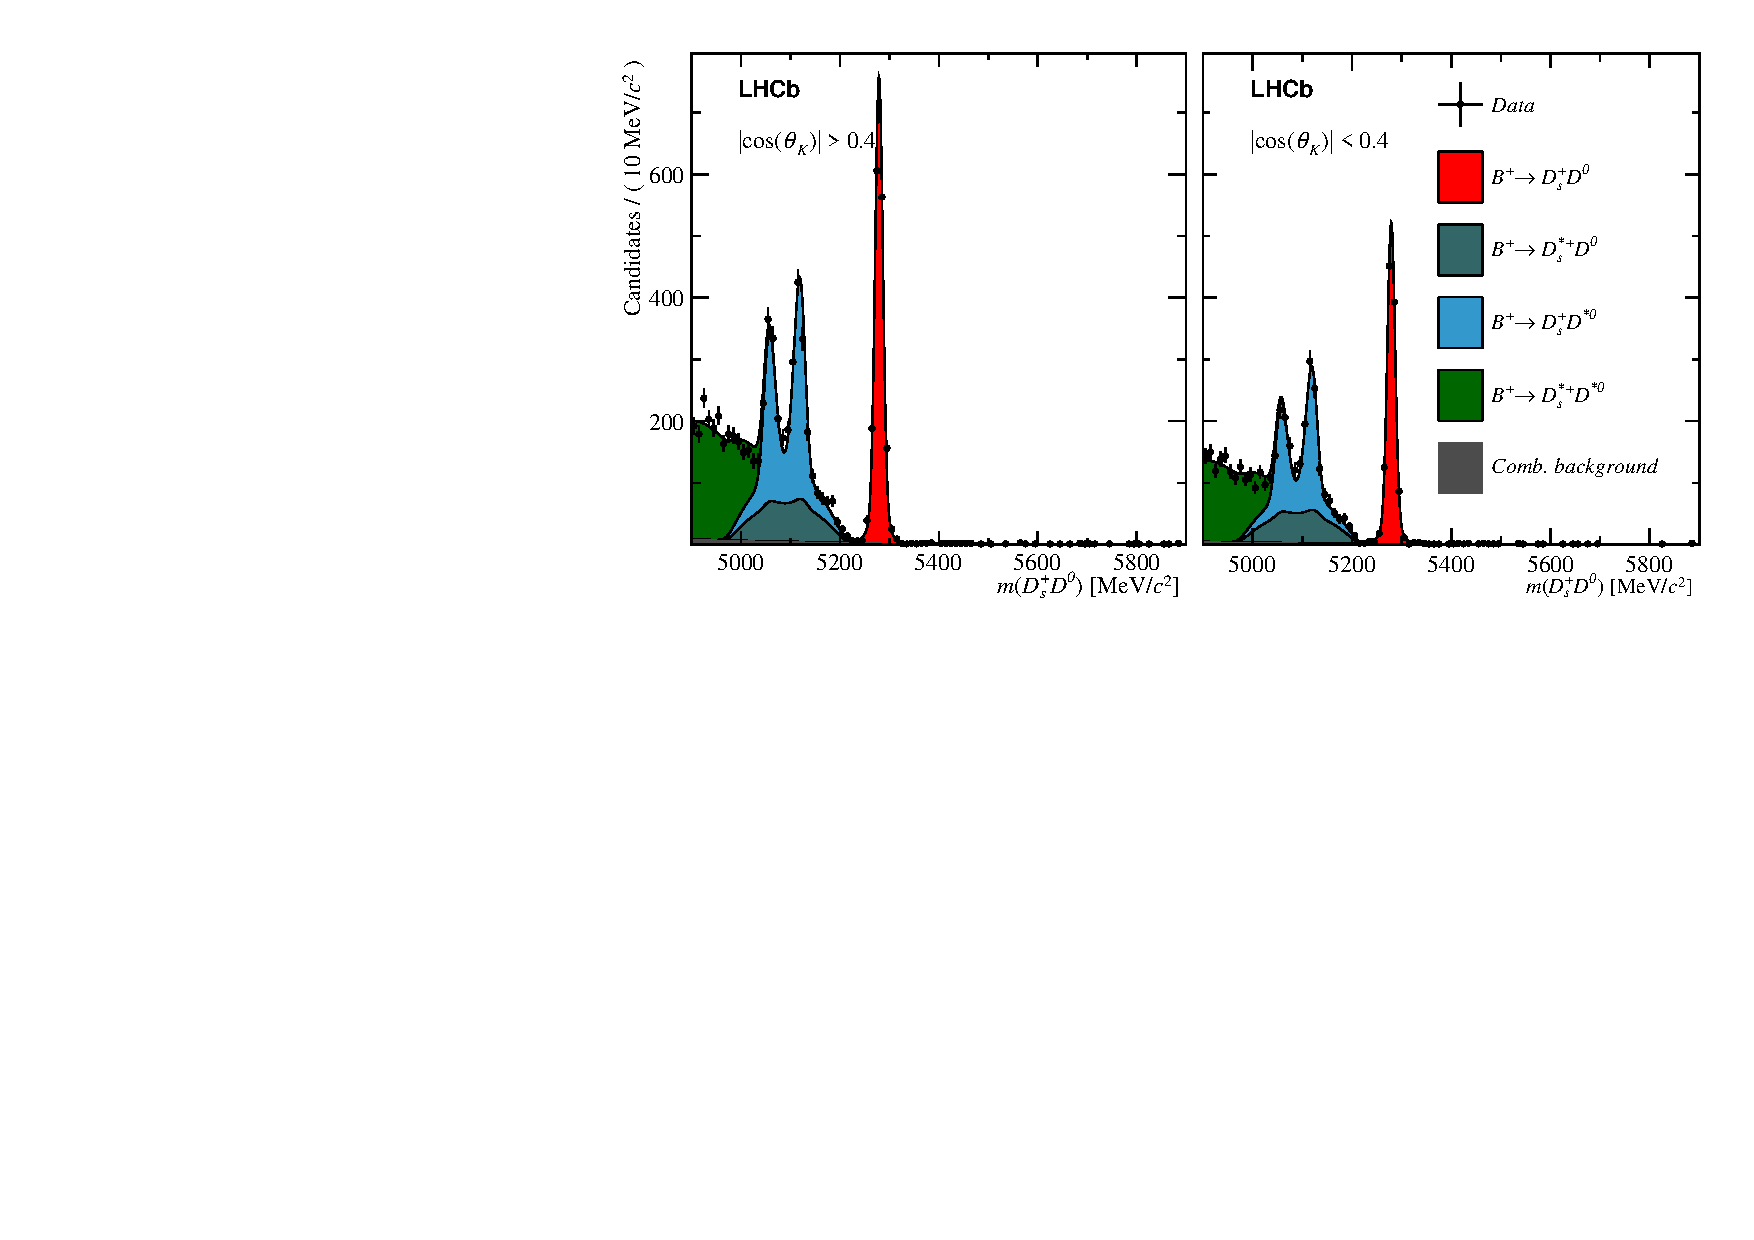
\includegraphics[width=1.0\textwidth]{figs/Appendix_FitCategories/canvas_DsD0_merged_both_summed_splitHel_splitKKPi_s21_s21r1_s24_s26.pdf}
    \end{subfigure}
    \caption{Invariant mass fits to \decay{\Bp}{\Dsp\Dzb} candidates}
\end{figure}
%%%%%%%%%%%%%%%%%%%%%%%%%%%%%%%%%%%%%%%%%%%%%%%%%%%%%%%%%%


%%%%%%%%%%%%%%%%%%%%%%%%%%%%%%%%%%%%%%%%%%%%%%%%%%%%%%%%%%
\begin{figure}[!h]
    \centering
    \begin{subfigure}[t]{1.0\textwidth}
        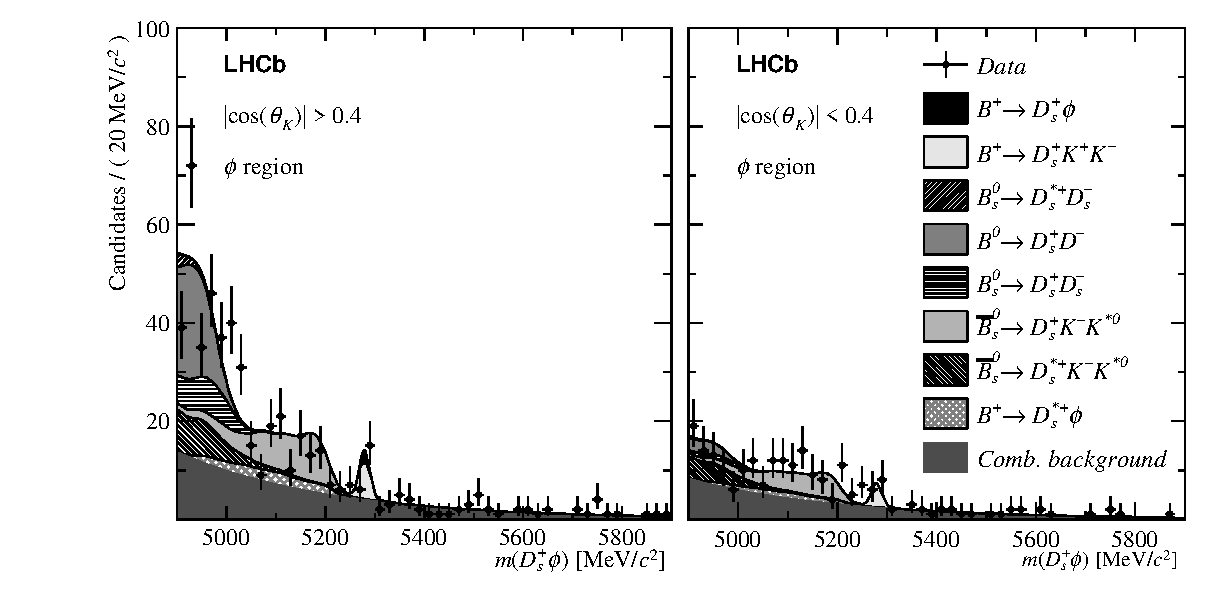
\includegraphics[width=1.0\textwidth]{figs/B2DsPhi/Fig4a.eps}
    \end{subfigure}
    \begin{subfigure}[t]{1.0\textwidth}
        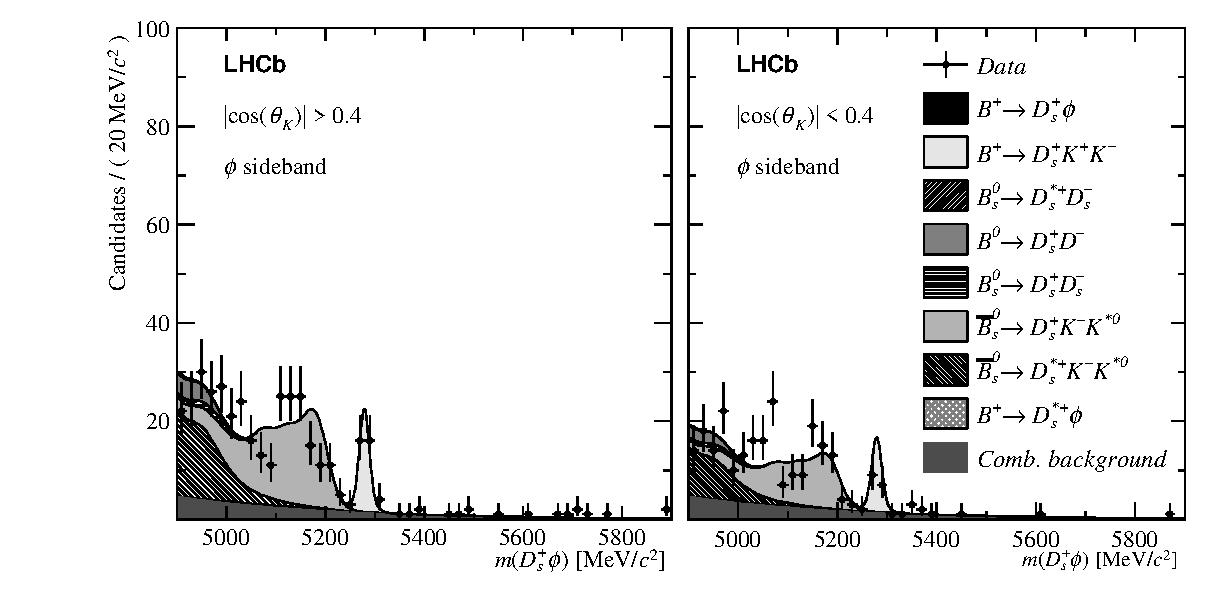
\includegraphics[width=1.0\textwidth]{figs/B2DsPhi/Fig4b.eps}
    \end{subfigure}
    \caption{Invariant mass fits to \decay{\Bp}{\Dsp\phiz} candidates}
\end{figure}
%%%%%%%%%%%%%%%%%%%%%%%%%%%%%%%%%%%%%%%%%%%%%%%%%%%%%%%%%%



\section{Efficiency corrections}
\label{sec:B2DsPhi_effcorrections}


{\color{Red}
\begin{itemize}
\item Assume pseudo two body decay, therefore simple ratio  
\end{itemize}
}

\section{Systematic uncertainties}
\label{sec:B2DsPhi_systuncertainy}



\section{Results}
\label{sec:B2DsPhi_results}

{\color{Red}
\begin{itemize}
\item Copy most of results section from paper
\end{itemize}
}

The fit to $\decay{\Bp}{\Dsp\phiz}$ candidates finds a total yield of $N(\decay{\Bp}{\Dsp\phiz}) = 5.3 \pm 6.7$, summed across all categories and \Dsp meson decay modes. 
A yield of $N(\decay{\Bp}{\Dsp\Km\Kp}) = 65 \pm 10 $ is found, consistent with the yield obtained from the full $\decay{\Bp}{\Dsp\Kp\Km}$ measurement. 
The branching fraction for $ \decay{\Bp}{\Dsp\phiz}$ decays is calculated as

\begin{equation}
\mathcal{B}(\decay{\Bp}{\Dsp\phiz}) = R \times \frac{\mathcal{B}(\decay{\Dzb}{\Kp\Km})}{\mathcal{B}(\decay{\phi}{\Kp\Km})} \times \mathcal{B}(\decay{\Bp}{\Dsp\Dzb}),
\label{eq:branching_fraction_calc}
\end{equation}
where the branching fraction $\mathcal{B}(\decay{\phi}{\Kp\Km})= 0.489 \pm 0.005$ has been used~\cite{PDG2016}. 

The free variable $R$ is defined to be the ratio of the signal and normalisation yields, corrected for the selection efficiencies.
The yield of signal candidates in each \Dsp mode is constructed from $R$ and the normalisation yield for the given \Dsp decay mode, $N(\decay{\Bp}{\Dsp\Dzb})$. The product of these two quantities is corrected by the ratio of selection efficiencies

\begin{equation}
N(\decay{\Bp}{\Dsp\phiz}) = R \times N(\decay{\Bp}{\Dsp\Dzb}) \times \frac{\epsilon(\decay{\Bp}{\Dsp\phiz})}{\epsilon(\decay{\Bp}{\Dsp\Dzb})}.
\label{eq:branching_fraction_R}
\end{equation}

The simultaneous fit measures a single value of $R$ for all \Dsp decay mode categories. From an ensemble of pseudoexperiments, $R$ is distributed normally. It can be written as the ratio of signal and normalisation branching fractions using Eq.~{\ref{eq:branching_fraction_calc}. The value is determined to be 

\begin{equation*}
R = \frac{\mathcal{B}(\decay{\Bp}{\Dsp\phiz})}{\mathcal{B}(\decay{\Bp}{\Dsp\Dzb})}\times \frac{\mathcal{B}(\decay{\phi}{\Kp\Km})}{\mathcal{B}(\decay{\Dzb}{\Kp\Km})} =(1.6^{+2.2}_{-1.9}\pm 1.1) \times 10^{-3}, 
\end{equation*}
where the first uncertainty is statistical and the second systematic. This corresponds to a branching fraction for $\decay{\Bp}{\Dsp\phiz}$ decays of

\begin{equation*}
\mathcal{B}(\decay{\Bp}{\Dsp\phiz}) = (1.2^{+1.6}_{-1.4} \pm 0.8  \pm 0.1)\times 10^{-7},
\label{eq:branching_fraction}
\end{equation*}
where the first uncertainty is statistical, the second systematic, and the third results from the uncertainty on the branching fractions $\mathcal{B}(\decay{\Bp}{\Dsp\Dzb})$, $\mathcal{B}(\decay{\phi}{\Kp\Km})$ and $\mathcal{B}(\decay{\Dzb}{\Kp\Km})$. Considering only the statistical uncertainty, the significance of the $\decay{\Bp}{\Dsp\phiz}$ signal is 0.8 standard deviations ($\sigma$). 




\subsection{Limit setting}
\label{sec:B2DsPhi_limitsetting}

{\color{Red}
\begin{itemize}
\item Document all methods attemped
\item CLs plots
\item likelihood
\item FC bands
\item Table of comparison 
\end{itemize}
}

%%%%%%%%%%%%%%%%%%%%%%%%%%%%%%%%%%%%%%%%%%%%%%%%%%%%%%%%%%
\begin{figure}[!h]
    \centering
        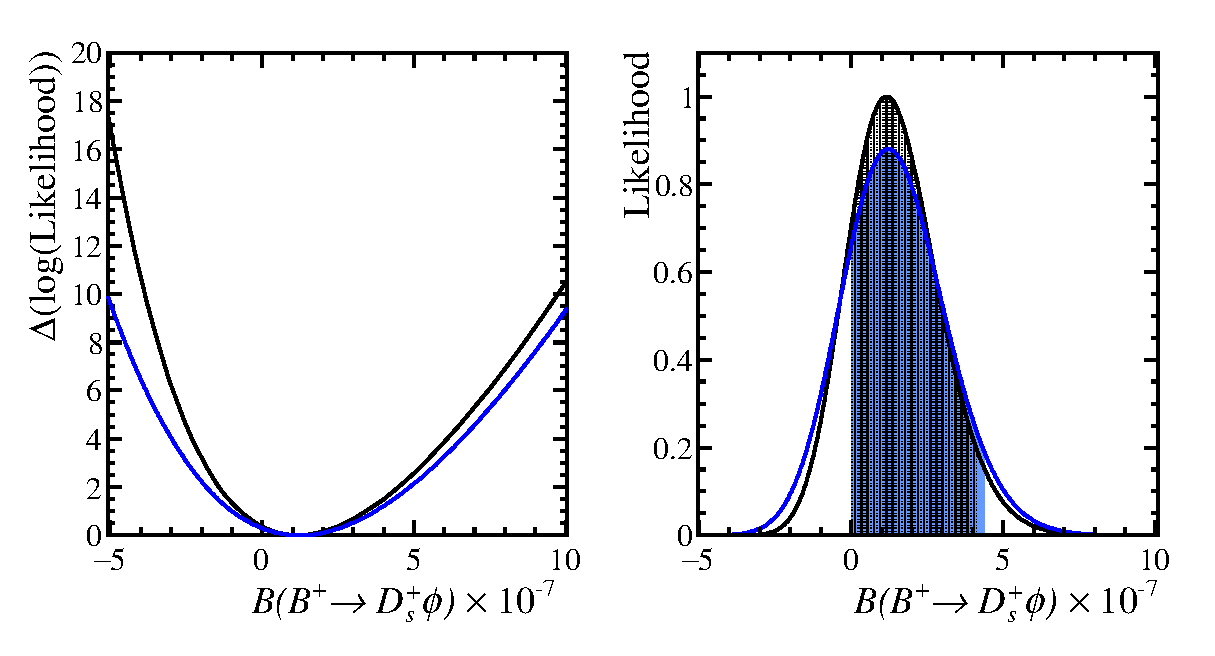
\includegraphics[width=1.0\textwidth]{figs/B2DsPhi/Likelihood_limits.eps}
        \caption{Bayesian profile likelihood limit determination}
    \label{fig:limit_likelihood}   
\end{figure}
%%%%%%%%%%%%%%%%%%%%%%%%%%%%%%%%%%%%%%%%%%%%%%%%%%%%%%%%%%

%%%%%%%%%%%%%%%%%%%%%%%%%%%%%%%%%%%%%%%%%%%%%%%%%%%%%%%%%%
\begin{figure}[!h]
    \centering
        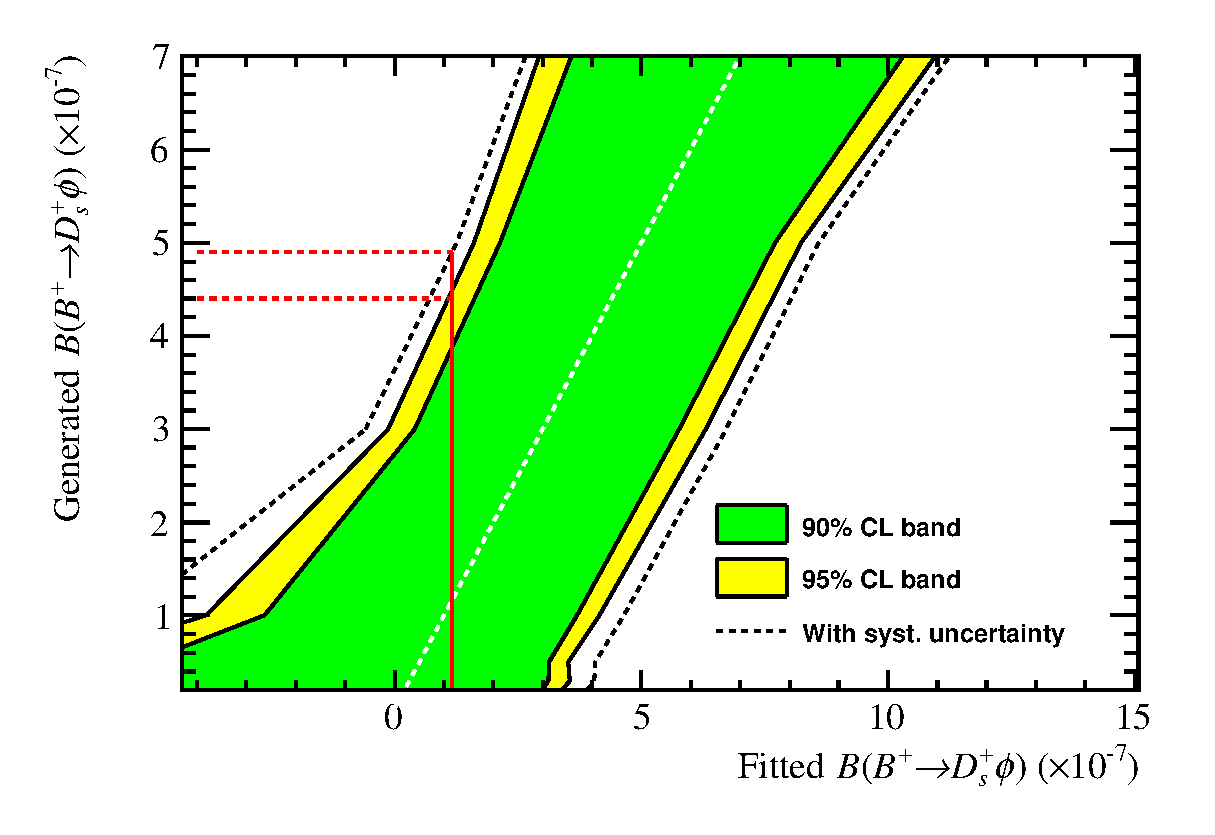
\includegraphics[width=0.8\textwidth]{figs/B2DsPhi/Sensitivity_plot.eps}
        \caption{CLs limit determination}
    \label{fig:limit_cls}   
\end{figure}
%%%%%%%%%%%%%%%%%%%%%%%%%%%%%%%%%%%%%%%%%%%%%%%%%%%%%%%%%%

